\documentclass[a4paper,12pt]{article}
\usepackage{amsmath}
\usepackage{amssymb}
\usepackage[polish]{babel}
\usepackage{polski}
\usepackage[utf8]{inputenc}
\usepackage{indentfirst}
\usepackage{geometry}
\usepackage{array}
\usepackage[pdftex]{color,graphicx}
\usepackage{subfigure}
\usepackage{afterpage}
\usepackage{setspace}
\usepackage{color}
\usepackage{wrapfig}
\usepackage{listings}
\usepackage{datetime}

\renewcommand{\onehalfspacing}{\setstretch{1.6}}

\geometry{tmargin=2.5cm,bmargin=2.5cm,lmargin=2.5cm,rmargin=2.5cm}
\setlength{\parindent}{1cm}
\setlength{\parskip}{0mm}

\newenvironment{lista}{
\begin{itemize}
  \setlength{\itemsep}{1pt}
  \setlength{\parskip}{0pt}
  \setlength{\parsep}{0pt}
}{\end{itemize}}

\newcommand{\linia}{\rule{\linewidth}{0.4mm}}

\definecolor{lbcolor}{rgb}{0.95,0.95,0.95}
\lstset{
    backgroundcolor=\color{lbcolor},
    tabsize=4,
  language=C++,
  captionpos=b,
  tabsize=3,
  frame=lines,
  numbers=left,
  numberstyle=\tiny,
  numbersep=5pt,
  breaklines=true,
  showstringspaces=false,
  basicstyle=\footnotesize,
  identifierstyle=\color{magenta},
  keywordstyle=\color[rgb]{0,0,1},
  commentstyle=\color{Darkgreen},
  stringstyle=\color{red}
  }

\begin{document}

\noindent
\begin{tabular}{|c|p{11cm}|c|} \hline 
Grupa 6 & Dariusz Szczupak, Kamil Wanat & \ddmmyyyydate\today \tabularnewline
\hline 
\end{tabular}

\section*{Zadanie 1 - Rozmycie Gaussa w OpenMP}

Celem zadania jest program oparty na algorytmie Gaussa mający na celu rozmycie danego zdjęcia. Zadanie wykonane w technologii OpenMP. "Gauss 2" - to użyta wersja filtru danego w dołączonym do treści zadania linku. Maska w danym filtrze wygląda następująco:

\begin{lstlisting}
int mask[5][5] = {{1,1,2,1,1}, {1,2,4,2,1}, {2,4,8,4,2}, {1,2,4,2,1}, {1,1,2,1,1}
};
\end{lstlisting}

Do obliczenia wartości z których składa się każdy piksel(Red, Green, Blue), potrzebne są punkty otaczające go. Każdy taki piksel ma jakąś wage, która z kolei zapisana jest w masce filtra. Liczymy sume ważoną kolejnych pixeli i jego sąsiadów, kolejnie dzielimy taką sumę przez sumę całej maski. Filtrowanie obrazu następuje oddzielnie dla każdej wartości z której składa się pixel. W metodzie filtrowania Gaussa znaczenie wartości pixela jest największe w punkcie, który jest liczony i zmniejsza się wraz z oddalaniem się od niego. Poniżej część programu która ulega zrównolegleniu:


\begin{lstlisting}
  #pragma omp parallel for shared(img, imgScore) private(x, y , column, row, R, G, B) num_threads(n_thr) schedule(static) 
  for(row = 2; row < rows-2; row++) 
  {
    for(column = 2; column < columns-2; column++)
    {
      int startA = row -2;
      int startB = column -2;
      Vec3b &pixelResult = imgScore.at<Vec3b>(startA, startB); 
      R = 0;
      G = 0;
      B = 0;
      for(x=0; x < 5; x++) 
        for(y=0; y < 5; y++){
          Vec3b pixelSource = img.at<Vec3b>(startA + x, startB + y);
                    R += pixelSource.val[0] * mask[x][y]; 
                    G += pixelSource.val[1] * mask[x][y]; 
                    B += pixelSource.val[2] * mask[x][y]; 
        }
            pixelResult.val[0] = R/SumMask;  
            pixelResult.val[1] = G/SumMask;
            pixelResult.val[2] = B/SumMask;
    }
  }

\end{lstlisting}

Do zrównoleglenia użyliśmy dyrektyw shared oraz private z OpenMP. Zmienne przechowujące obrazek oraz obrazek wynikowy ustawilismy jako zmienne wspólne, czyli dostępne dla wszystkich wątków, natomiast zmienne x, y, row, column - będące licznikami w pętli - indeksy maski oraz kolejne punkty na obrazie, są zmiennymi prywatnymi. Każda z nich jest przypisana do jednego wątku. Poniżej wykresy pomiarów czasu dla różnej ilości wątków:


\begin{wrapfigure}{r}{0.5\textwidth}
  \vspace{-20pt}
  \begin{center}
  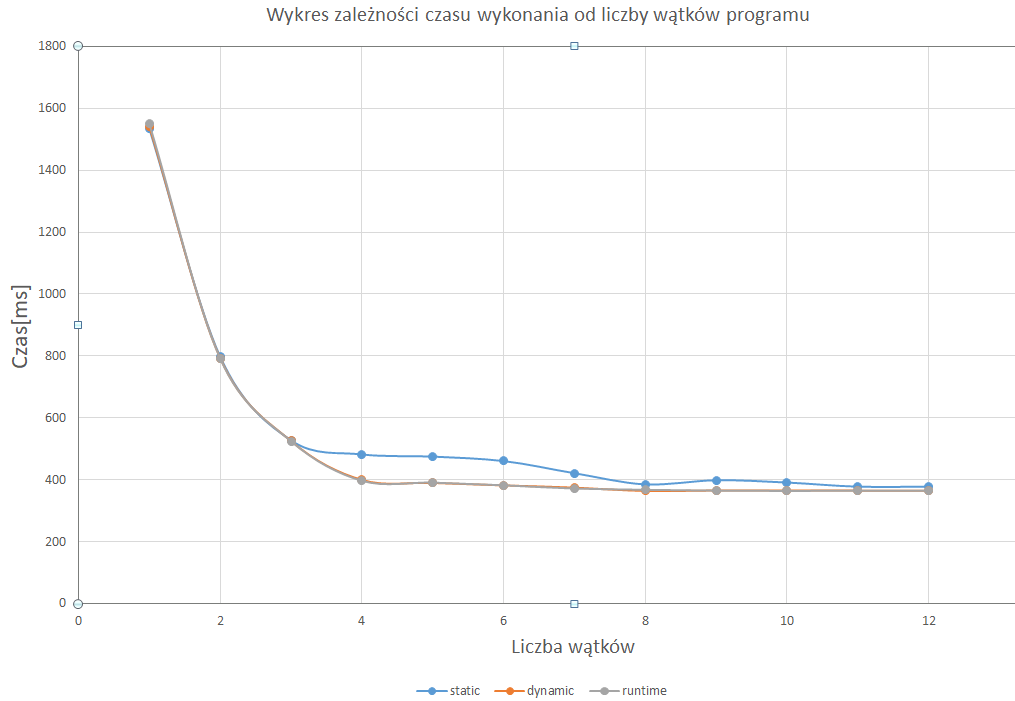
\includegraphics[width=0.45\textwidth]{wykres.PNG}
  \end{center}
  \vspace{-20pt}
  \caption{Wykres zależności czasu od liczby wątków}
  \vspace{-10pt}
\end{wrapfigure}

\begin{figure}[!hbp]
  \centering
  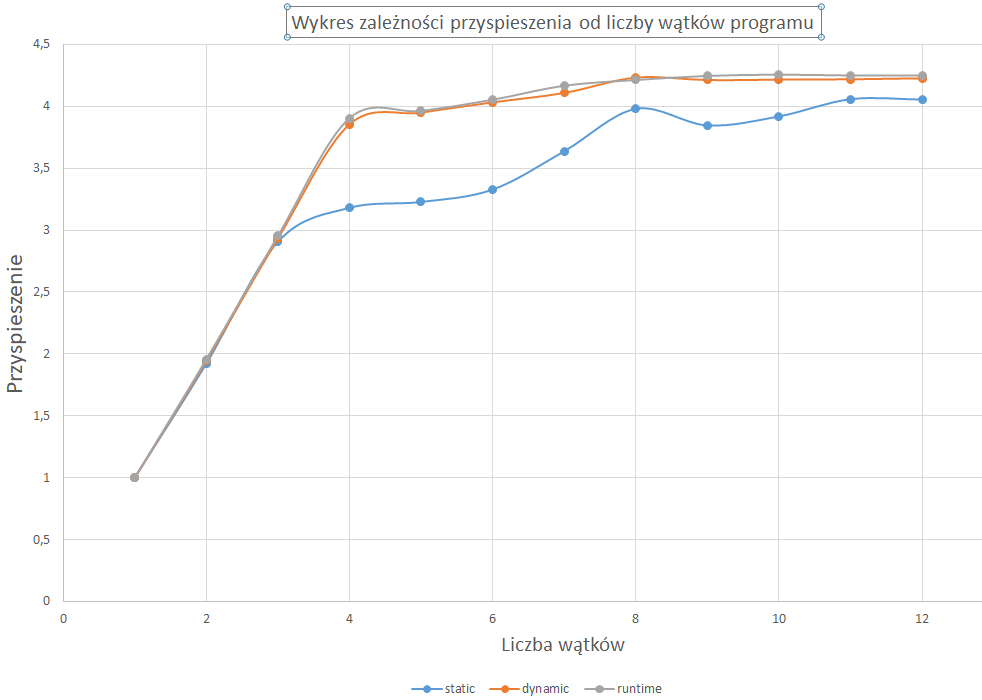
\includegraphics[width=0.7\textwidth]{wykres1.PNG}
  \caption{Wykres zależności liczby wątków od przyśpieszenia}
\end{figure}

Z powyższych wykresów można wywnioskować że czas obliczeń na całym przedziale nieznacznie spada. Załamania występują dla 4 wątków, oraz dla 8-9 wątków co ma zapewnie związek z hyper-threading i liczbą rdzeni na serwerze cuda. Najlepszą wydajność mamy dla 9 wątków(ponad 4 sekundy), natomiast najgorszą przy załamaniu dla 4 wątków.
Na wykresie przyśpieszenia można zauważyć że dla 9 wątków mamy najlepsze przyśpieszenie, które jest ponad 1,2 - krotne.    

Dane przeprowadzanych testów:
\begin{lista}
 \item Wzięto pod uwagę średnią pomiarów czasów wykonania programu dla liczby wątków z przedziału od 1 do 12. Program był uruchamiany dla obrazka ściągniętego z przestworzy internetów w rozdzielczośći 1920x1200px.
 \item Do mierzenia czasu wykorzystano omp\_get\_wtime.
 \item Do wczytania obrazu wykorzystano bibliotekę OpenCV .
 \item Testy zostały wykonane na serwerze cuda.iti.pk.edu.pl . 
\end{lista}
 
Zapoznaliśmy się ze środowiskiem OpenMP. Zadanie udało się wykonać w całości. Dostaliśmy kilka pomiarów czasów, które były niespójne z pozostałą częścią obliczeń(kilka wyników dla dwóch może trzech wątków) i zostały one uśrednione - wynikło to prawdopodobnie z równoległego wykonywania programów przez kilka osób naraz na serwerze. Wniosek nasuwa się taki, iż za pomocą OpenMP można przyspieszyć czas obliczeń algorytmu rozmycia Gaussa. Najlepsze wyniki osiągnięto dla ilości wątków zbliżonej do ilości rdzeni procesora na serwerze CUDA. 


\end{document}

